\documentclass{templateNote}

\begin{document}

% \imagenlogoD{img/LogoNGM.png}
% \linklogoD{https://github.com/NicoxlkboUni}
% \universidad{Universidad del Bío-Bío}
\imagenlogoU{img/LogoElNube.png}
\linklogoU{https://github.com/MarceloPazPezo}
\linkQRDoc{https://github.com/MarceloPazPezo/MyRepo/tree/main/Icinf}
\titulo{Guía de ejercicios (ExControl 1)}
\asignatura{Administración y Programación de Base de Datos}
\autor{
    \indent
    Marcelo \textsc{Paz}
}
\vDoc{1.0.0}

% Metadatos del PDF
\title{[\asignatura]-\titulo}
\author{
    \autor
}
\portada
\margenes % Crear márgenes
\section{Ex-Control 1}
\begin{enumerate}
    \item \textbf{(0.5 pts) ¿Cuál es la diferencia entre un bloqueo de dos fases y un bloqueo de dos fases estricto?}

    \textcolor{blue}{   
        Bloqueo de dos fases estricto, se deben solicitar todas las solicitudes de candados, mientras se ocupan, y se liberan al final, mientras que el de dos fases, debe solicitar todos los candados necesarios, pero luego puede ir liberando, sin tener que esperar por el commit final.
    }
    \item \textbf{(0.5 pts) Un trigger está conpuesto por tres partes, ¿Cuáles son? (Solo nombrarlas)}
    \\ \textcolor{blue}{
    Las partes de un trigger son:
    \begin{itemize}
        \item Evento.
        \item Condición.
        \item Acción.
    \end{itemize}
    }
    \item \textbf{(0.5 pts) Indicar cuáles son las consecuencias de estas tres acciones:}
    \begin{enumerate}
        \item \textbf{GRANT SELECT ON T TO luis WITH GRANT (ejecutada por A)}
        \\ \textcolor{blue}{\textit{'A'} le otorga permisos de lectura de la tabla \textit{'T'} a \textit{'luis'}, no hay problemas.}
        
        \item \textbf{GRANT INSERT ON T TO jose (ejecutada por luis)}
        \\ \textcolor{blue}{\textit{'luis'} le otorga permisos de insertar a \textit{'jose'}, sobre la tabla \textit{'T'}. El problema aqui, es que \textit{'luis'}, no tiene esos permisos, por ende, no se puede ejecutar la acción. \textit{'jose'} no recibe nada.}
        
        \item \textbf{REVOKE SELECT ON T FROM jose (ejecutada por A)}
        \\ \textcolor{blue}{\textit{'A'}, le quita los permisos a \textit{'jose'} sobre \textit{'T'}, pero como anteriormente no se le otorgo nada, tampoco se puede ejecutar.}
    \end{enumerate}

    \newpage
    \item \textbf{(0.5 pts) Indicar en un dibujo simple, las partes: Disco, sector, pista y bloque.}
    
    \begin{figure}[H]
        \centering
        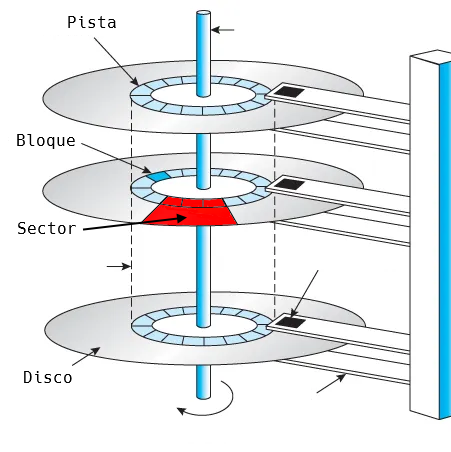
\includegraphics[width=1\textwidth]{img/DibujoDisco.png}
    \end{figure}
    \newpage
    \item \textbf{(1 pts) Considerar Megatron 777, con las siguientes características:}
    \begin{itemize}
        \item Existen 6 discos.
        \item 20\% de cada pista es usado para gaps.
        \item Cada sector es de 512 bytes y cada pista en promedio tiene 550 sectores.
        \item 100 tracks/pistas por superficies.
        \item El disco rota a 4000 RPM.
    \end{itemize}

    Si un block tuviera 30 sectores, cuanto tiempo tomaría transferir 3 bloques consecutivos (transfer time o tiempo de transferencia).
    \textcolor{blue}{
        \begin{itemize}
            \item \textbf{Paso 1: Calculamos la cantidad de sectores y gaps:}
            \begin{align*}
                3 \cdot 30 \text{ Sectores} + (3 \cdot 30 - 1) \text{ Gaps}
            \end{align*}
            \item \textbf{Paso 2: Calculamos cuantos grados son de gaps en un disco:}
            \begin{align*}
                \text{Gaps} = 360\text{°} \cdot \frac{20}{100} = 72\text{°}
            \end{align*}
            \item \textbf{Paso 3: Calculamos cuantos grados son de sectores en un disco:}
            \begin{align*}
                \text{Sectores} = 360\text{°} - 72\text{°} = 360\text{°} \cdot \frac{80}{100} = 288\text{°}
            \end{align*}
            \item \textbf{Paso 4: Calculamos cuantos grados son de un sector:} (Sabemos que el promedio de sectores son 550)
            \begin{align*}
                \text{Sector} = 288\text{°} \div 550 = 0.523\text{°}
            \end{align*}
            \item \textbf{Paso 5: Calculamos cuantos grados son de un gap:}
            \begin{align*}
                \text{Gap} = 72\text{°} \div 550 = 0.131\text{°}
            \end{align*}
            \item \textbf{Paso 6: Calculamos cuanto es una rotación en tiempo:}
            \begin{align*}
                1 \text{ rotación} = \frac{1}{4000} \cdot 60 \text{ segundos} = 0.015 \text{ segundos} = 15 \text{ ms}
            \end{align*}
            \item \textbf{Paso 7: Calculamos cuanto grados ocupan 3 bloques consecutivos:}
            \begin{align*}
                \text{3 Bloques consecutivos} &= (0.523\text{°} \cdot 90 \text{ Sectores}) + (0.131\text{°} \cdot 89 \text{ Gaps}) \\
                &= 47.07\text{°} + 11.659\text{°} = 58.729\text{°}
            \end{align*}
            \item \textbf{Paso 8: Calculamos cuanto tiempo toma transferir 3 bloques consecutivos:}
            \begin{align*}
                \text{tt} &= \left(\frac{58.729\text{°}}{360\text{°}}\right) \cdot 15 \text{ ms} \\
                &= 2.4470 \text{ ms}
            \end{align*}
        \end{itemize}
    }
    \item \textbf{(0.8 pts) Utilizando RAID 6, para múltiples fallas de disco. Si falla disco 1 y disco 6, recuperar para dejar estable nuevamente.}
    \begin{figure}[H]
        \centering
        \begin{tabular}{|c|}
            \hline
            \textbf{D1) 11110000} \\
            \hline
            \textbf{D2) 10101010} \\
            \hline
            \textbf{D3) 00111000} \\
            \hline
            \textbf{D4) 01000001} \\
            \hline
        \end{tabular}
    \end{figure}
    \begin{figure}[H]
        \centering
        \begin{tabular}{|c|c|c|c|c|c|c|}
            \hline
            1 & 2 & 3 & 4 & 5 & 6 & 7 \\ \hline
            1 & 0 & 1 & 1 & 1 & 0 & 0 \\
            1 & 1 & 0 & 1 & 0 & 1 & 0 \\
            0 & 1 & 1 & 1 & 0 & 0 & 1 \\ \hline
        \end{tabular}
    \end{figure}

    \begin{enumerate}
        \item Obtener discos de recuperación.
        \textcolor{blue}{
            \begin{align*}
                D5 &= D1 + D3 + D4 \\
                D6 &= D1 + D2 + D4 \\
                D7 &= D2 + D3 + D4
            \end{align*}
            \begin{equation*}
                \begin{array}{cc}
                    \begin{array}{ccccccccc}
                            & 1 & 1 & 1 & 1 & 0 & 0 & 0 & 0 \\
                            & 0 & 0 & 1 & 1 & 1 & 0 & 0 & 0 \\
                            & 0 & 1 & 0 & 0 & 0 & 0 & 0 & 1 \\ \hline
                        D5: & 1 & 0 & 0 & 0 & 1 & 0 & 0 & 1 \\
                    \end{array} &\hspace{1cm}
                    \begin{array}{ccccccccc}
                            & 1 & 1 & 1 & 1 & 0 & 0 & 0 & 0 \\
                            & 1 & 0 & 1 & 0 & 1 & 0 & 1 & 0 \\
                            & 0 & 1 & 0 & 0 & 0 & 0 & 0 & 1 \\ \hline
                        D6: & 0 & 0 & 0 & 1 & 1 & 0 & 1 & 1 \\
                    \end{array} \\[1.5cm]
                    \begin{array}{ccccccccc}
                            & 1 & 0 & 1 & 0 & 1 & 0 & 1 & 0 \\
                            & 0 & 0 & 1 & 1 & 1 & 0 & 0 & 0 \\
                            & 0 & 1 & 0 & 0 & 0 & 0 & 0 & 1 \\ \hline
                        D7: & 1 & 1 & 0 & 1 & 0 & 0 & 1 & 1 \\
                    \end{array} &
                \end{array}
            \end{equation*}
        }
        \item Recuperar discos fallados.
        
        \textcolor{blue}{
            \begin{align*}
                D1 &= D5 + D3 + D4 \\
            \end{align*}
            \begin{equation*}
                \begin{array}{ccccccccc}
                        & 1 & 0 & 0 & 0 & 1 & 0 & 0 & 1 \\
                        & 0 & 0 & 1 & 1 & 1 & 0 & 0 & 0 \\
                        & 0 & 1 & 0 & 0 & 0 & 0 & 0 & 1 \\ \hline
                    D1: & 1 & 1 & 1 & 1 & 0 & 0 & 0 & 0 \\
                \end{array}
            \end{equation*}
            Y para el disco 6:
            \begin{align*}
                D6 &= D1 + D2 + D4 \\
            \end{align*}
            \begin{equation*}
                \begin{array}{ccccccccc}
                        & 1 & 1 & 1 & 1 & 0 & 0 & 0 & 0 \\
                        & 1 & 0 & 1 & 0 & 1 & 0 & 1 & 0 \\
                        & 0 & 1 & 0 & 0 & 0 & 0 & 0 & 1 \\ \hline
                    D6: & 0 & 0 & 0 & 1 & 1 & 0 & 1 & 1 \\
                \end{array}
            \end{equation*}    
        }
    \end{enumerate}

    \item \textbf{(0.8 pts) Suponer que las llaves son Hash en secuencias de 4 bits. Los bloques pueden contener 2 registros. Si se comienza con una tabla hash con dos bloques vacios (correspondientes a 0 y 1). Mostrar la organización depues de insertar con llaves: 1111,0001,0000,1110 y 0100. Utilizando Hash extensible.}
    \item \textbf{(0.6 pts) Considere el siguiente árbol B (Figura A), inicialmente con el conjunto de claves C cuyo grado mínimo es 3. Eliminar del árbol el número 60.}
    \item \textbf{(0.6 pts) Considere el siguiente árbol B (Figura B), inicialmente con el conjunto de claves C cuyo grado mínimo es 4. Insertar en el árbol presentado el número 66.}
    \item \textbf{BONUS (0.2 pts): ¿Qué indica la cláusula FOR EACH ROW?}
\end{enumerate}


    
    
    
\end{document}